\documentclass[paper=a4]{article}
\usepackage{ucs}
\usepackage[utf8x]{inputenc}
\usepackage[T1]{fontenc}
\PreloadUnicodePage{0}
\usepackage{xspace}
\usepackage{array}
\usepackage[hmargin=3.5cm,vmargin=2.7cm]{geometry} 
\usepackage{graphicx}
\usepackage{mathtools}

\renewcommand{\contentsname}{Innhold}

\begin{document}
\title{
	\vspace*{10em}
	
\includegraphics[width=1.00\textwidth]{images/logo.png}
	\vspace*{3em}
}
\author{\textbf{Spillmanual} \\
Team Dank \\
Universitetet i Bergen \\
Informatikk}
\maketitle
\newpage
\tableofcontents
\newpage

\section{Introduksjon}
Dette er et spill tiltenkt datamaskiner der spillere kjemper om å overleve lengre enn sine motstandere. Det kan være opp til 4 spillere, men minimum 2. 
Spillet er et rundebasert 2D-platform strategi artilleri spill. Spillerne kan bevege seg i 30 sekunder for å posisjonere seg. 
Etter alle har posisjonert seg vil de ha muligheten til å sikte seg inn på fiender med våpen som skyter matvarer. 
Disse matvarene er melk, gulrot, ost, cola, cupcake, donut, bløtkake, pizza, krone-is, brød, nudler, ostepop, potet, rødvin, seigemenn, sjokolade, sushi, vannmelon og wienerpølse, i skrivende stund. Flere kan bli implementert i senere versjoner.
Når man har truffet en fiende, vil denne fienden legge på seg det antall kalorier matvaren inneholder. 
Dersom spilleren kommer over en grense kalorier vil spilleren tape, og er ute av spillet. Den som overlever til slutt vil vinne spillet.


\section{Systemkrav og installasjon}

\subsection{Systemkrav}
\begin{itemize}
	\item{Ikke mindre 1 GB RAM}
	\item{Windows Vista/Linux 2.6.12/Mac OS X 10.4 eller nyere}
	\item{50 MB ledig plass for installasjon}
	\item{Java 8}
	\item{Tastatur og mus}
	\item{TeamDank anbefaler deg å ha en prosessor (2005+) med klokkefrekvens på 1.6 GHz eller bedre}
\end{itemize}

\subsection{Installasjon}
Du må først sørge for at du har installert den nyeste versjonen av Java og \\
for å kunne spille FoodFeud må du laste ned $foodfeud.jar$ filen. \\
Deretter åpner du filen som vanlig for å starte spillet.  
\newpage

\section{Spillinstruksjoner og -regler}

\subsection{Kontroll og instruksjoner}
Din primære spillinngangsenhet er tastaturet og musen, og kan gjøre følgende:
\begin{itemize}
	\item{Når du starter spillet må du først velge antall spillere ved å trykke på 2, 3 eller 4}
	\item{Deretter trykker du på hvilken rekkefølge spillerne skal starte rundene sine}
	\item{Du styrer din spiller med piltastene eller $A$ og $D$, du kan hoppe ved å trykke pil opp eller $W$}
	\item{For å kunne gå opp mange av bakkene må du hoppe samtidig som du går oppover}
	\item{For å skyte dine motstandere, sikter du deg inn med posisjonen av musen og trykker høyre museknapp for å skyte}
	\item{For at du skal være ferdig med din tur må du trykke på $space$} %TODO
	\item{Du kan pause spillet ved å gå til pausemenyen ved å trykke på tastaturknappen $ESC$, eller gå ut av spillet}
	\begin{itemize}
		\item{Å være på pausemenyen vil gi deg muligheten til å fortsette eller avslutte spillet.}
	\end{itemize}
\end{itemize}

\subsection{Objekt-interaksjon}
Det er forskjellige matvarer som blir brukt som skudd i FoodFeud, skaden blir bestemt av antall kalorier matvaren inneholder. Noen eksempler er:

{\renewcommand\labelitemi{}
\begin{itemize}
	\item 
\includegraphics[scale = 0.3]{images/Ananas.png} \textbf{Ananas}
	\item 
\includegraphics[scale = 0.4]{images/Melkekartong.png} \textbf{Melkekartong}
	\item 
\includegraphics[scale = 0.5]{images/Sushi.png} \textbf{Sushi}
\end{itemize}

Det finnes 4 forskjellige spillere:

\begin{itemize}
	\item 
\includegraphics[scale = 0.3]{images/elvis.png} \textbf{Geir Karltveit}
	\item 
\includegraphics[scale = 0.3]{images/kimk.png} \textbf{Gertrude Skogsheim}
	\item 
\includegraphics[scale = 0.3]{images/cowboy.png} \textbf{Per-Ole Nordskog}
	\item 
\includegraphics[scale = 0.3]{images/rockboy.png} \textbf{Knut-Roger Regeltun}
\end{itemize}
}

\newpage
\section{Bilder}
	\begin{center}
		{\renewcommand\labelitemi{}
			\begin{itemize}
				\item{\makebox[13.5cm]{
\includegraphics[width=1.00\textwidth]{images/startmenu.png}}}
				\item {\hfil Figure 1. Hovedmeny} 
				\bigskip
				\bigskip
				\bigskip
				\item{\makebox[13.5cm]{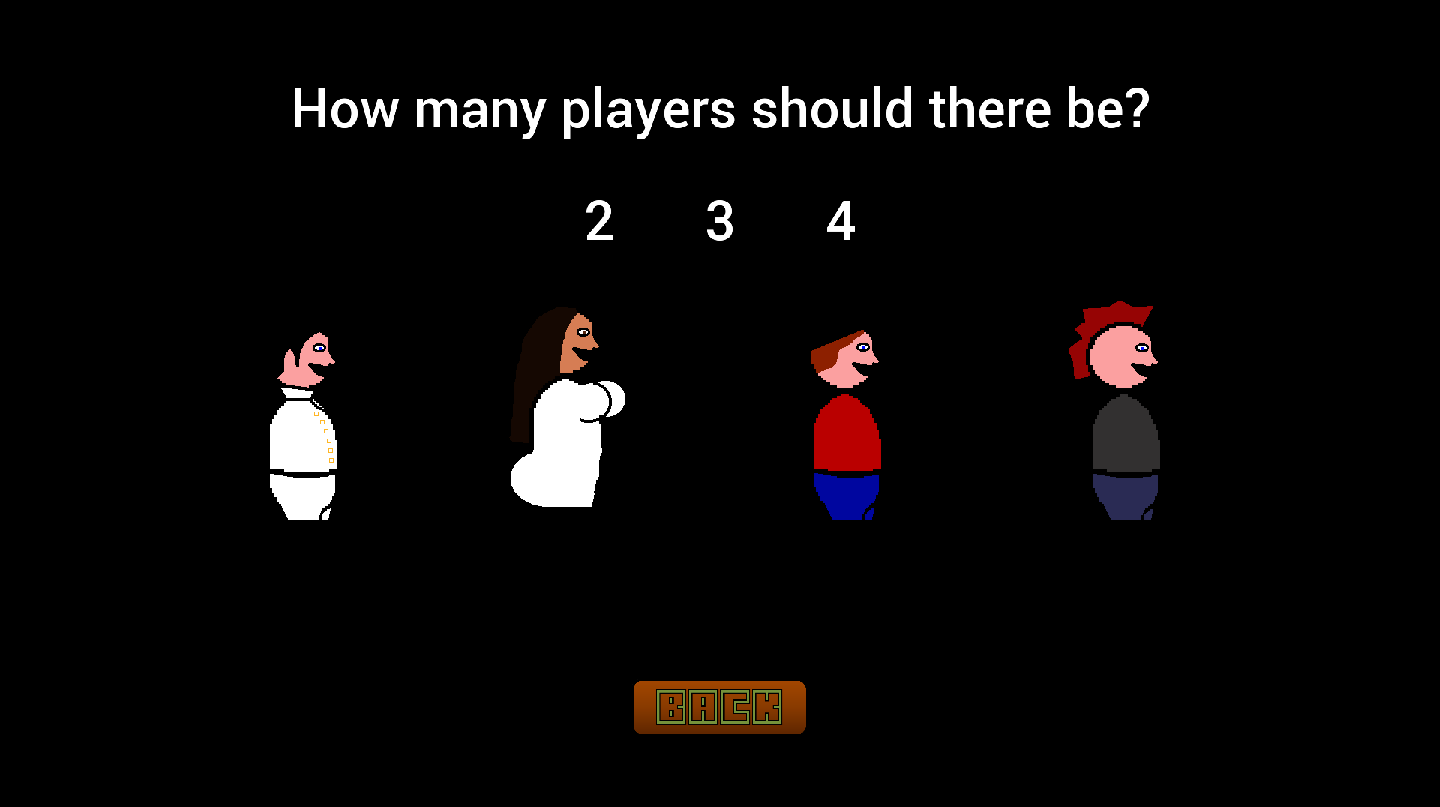
\includegraphics[width=1.00\textwidth]{images/setupmenu.png}}}
				\item {\hfil Figure 2. Oppsetsmeny} 
				\bigskip
				\bigskip
				\bigskip
				\item{\makebox[13.5cm]{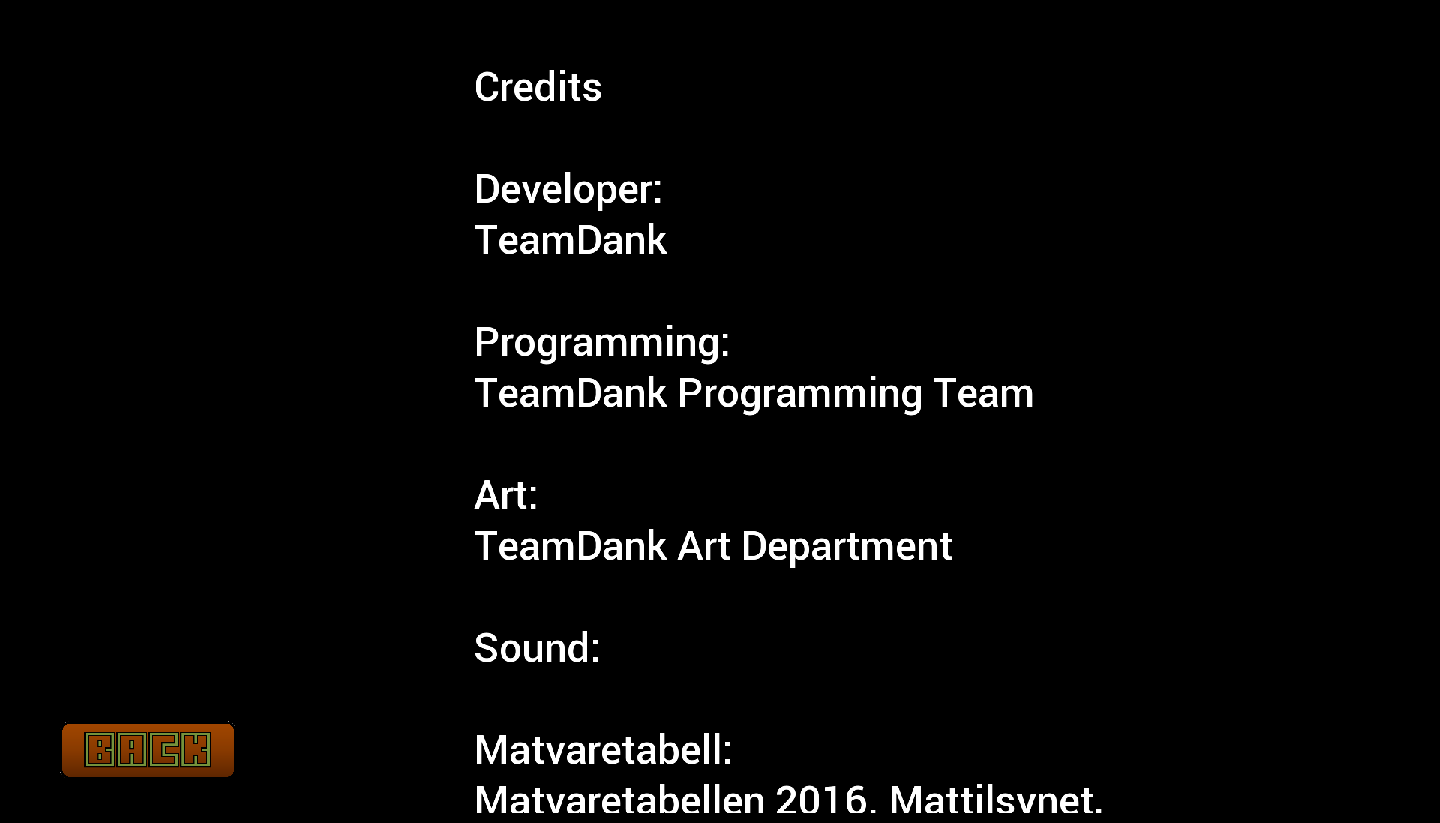
\includegraphics[width=1.00\textwidth]{images/creditmenu.png}}}
				\item {\hfil Figure 3. Kreditering} 
				\bigskip
				\bigskip
				\bigskip
				\item{\makebox[13.5cm]{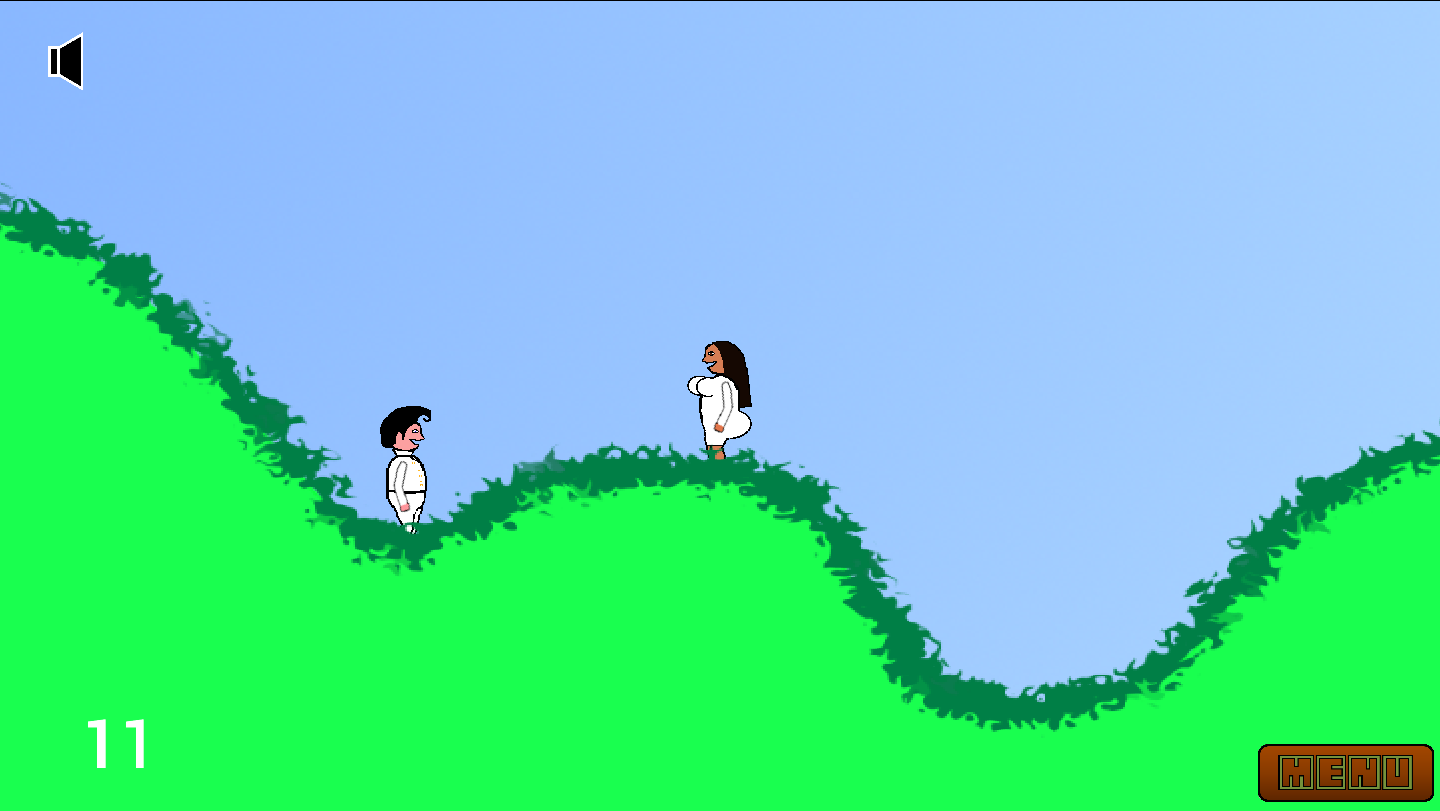
\includegraphics[width=1.00\textwidth]{images/duel.png}}}
				\item {\hfil Figure 4. Duell mellom Geir Karltveit og Gertrude Skogsheim} 
				\bigskip
				\bigskip
				\bigskip
				\item{\makebox[13.5cm]{
\includegraphics[width=1.00\textwidth]{images/pausemenu.png}}}
				\item {\hfil Figure 5. Pausemeny} 
				\bigskip
				\bigskip
				\bigskip
				\item{\makebox[13.5cm]{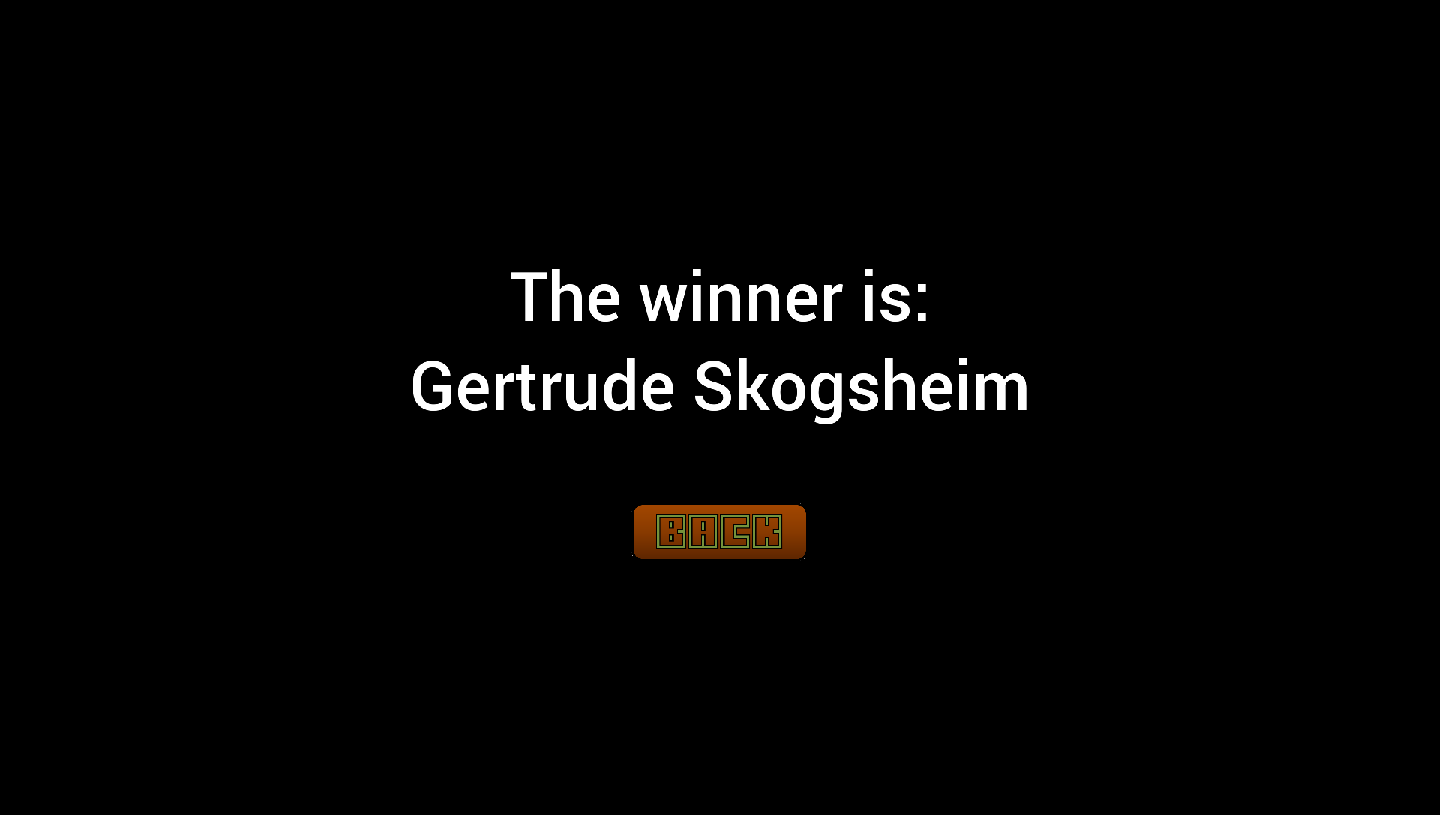
\includegraphics[width=1.00\textwidth]{images/winmenu.png}}}
				\item {\hfil Figure 5. Vinner} 
				\bigskip
				\bigskip
				\bigskip
			\end{itemize}
		}
	\end{center}

\newpage
\section{Credits}

\begin{center} 
\textbf{TeamDank}\\ \

\textbf{Utvikler team:}\\
TeamDank Programming Team\\ \

\textbf{Grafikk:} \\
TeamDank Art Department \\ \

\textbf{Matvaretabell:} \\ 
Matvaretabellen 2016. \\
Mattilsynet, Helsedirektoratet og Universitetet i Oslo \\ http://www.matvaretabellen.no \\ \

\textbf{Lyder:} \\ 
Lyder brukt fra freesound: \\ \

Hoppelyd av $kfatehi$ \\ https://www.freesound.org/people/kfatehi/sounds/363921/ \\ \

Løpelyd av $stintx$ \\ https://www.freesound.org/people/stintx/sounds/107624/ \\ \

Bakgrunnslyd av $Mrthenoronha$ \\ https://www.freesound.org/people/Mrthenoronha/sounds/369920/ \\ \

Projektil treffer person av $MonkeyFacebook532$ \\ https://www.freesound.org/people/MonkeyFacebook532/sounds/250082/ \\ \

Kastelyd av $denao270$ \\ https://www.freesound.org/people/denao270/sounds/346373/ \\ \

\

\textbf{Utviklere}: \\
Peter Andre Johansen \\
Håvar Eggereide \\
Kenneth Apeland \\
Philip Thao Hoang \\
Markus Johan Ragnhildstveit \\
Torbjørn Ola Sunnarvik Moen \\
Elias Refvem Siljan \\
Sturle Fraga Elvestad \\
Eirik Strøm \\
Amund Lindberg \\
Ole Magnus Lie \\
Bjørnar Herland \\ \

\textbf{Grafikk:} \\
Malin Øien \\
Emilia Botnen Van den Bergh \\ \

\textbf{Coach:} \\
Gunnar Schulze \\ \ 

\textbf{Juridisk Team:} \\ 
Anna Fossen-Helle \\ \

\textbf{Spillidé:} \\
$Team 1\textunderscore7$\\
Tony H. Abaz \\
Eirik Rye Ahlsen \\
Emilia Botnen

\end{center}

\end{document}